\section{Introduction}
As IO bandwidth continues to be significantly less than compute bandwidth in-situ methods have become essential. We hope to address the inverse relationship of IO and compute time by focussing on the intersection of two domains in which there is an increasing need for in situ solutions in both applied and research communities, namely, scientific visualisation and machine learning applications. The purpose of this project is then to offer a solution which provides the means necessary to design machine learning implementations at scale and in situ to aid or be the basis of visualisation and simulation tasks. We accomplish this by providing read, write and in place data transfer functionality between learning models and visualisation task implementations. 

In this work we demonstrate an example application of PAVE's platform by employing a neural network for real time rendering and accurate light transport simulation within the framework of Python, specifically PyTorch, made compatible for distributed systems and high performance computing (HPC). The provided model is a coalescence of the Visualisation Toolkit fit for Massively threaded architectures (VTK-m), Python, an increasingly popular language within the machine learning community due to robust libraries for neural networks such as PyTorch, and Adios2, an adaptable unified IO framework for data management at scale. The resulting work accomplishes this combination by utilising VTK-m to construct a path trace rendering tool able to fluidly and efficiently communicate to a cGAN by means of Adios2 during training.   The resulting generative model serves as a real-time filter for rendering images and visual simulations accurately approximating indirect illumination and soft shadows with quality comparable to offline approaches. 

\begin{figure*}
    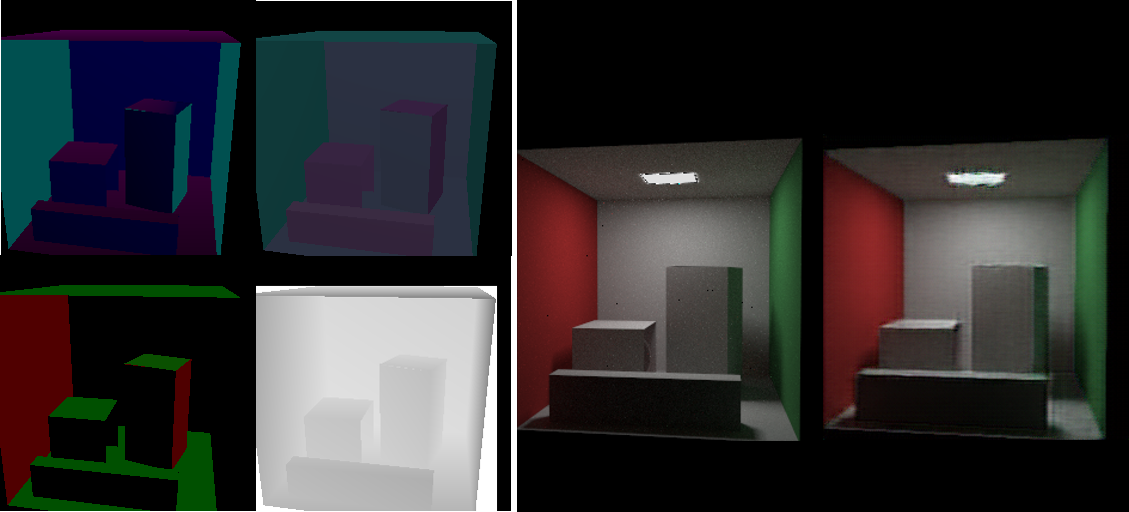
\includegraphics[width=\linewidth]{buffer_results_teaser}
    \caption{Rendered Conditional Geometry Buffers ({\bf left set}) and artificial rendering with conditional generative adversarial neural network ({\bf right couple}) comparing ground truth path traced rendering ({\bf left}) with image generated ({\bf right}).}
  \end{figure*}
